\documentclass{beamer-control}
\usepackage{beamer-control-singlefile}
\INCLUDEONLY{Feedback Design via Loop Shaping}
\begin{document}
\CONCEPT{Feedback Design via Loop Shaping}

\begin{SUMMARY}
\begin{itemize}
\item Design considerations
\item Lead and lag compensation
\end{itemize}
\vfill References:
\begin{itemize}
\item \astrom{§12.3}
\end{itemize}
\end{SUMMARY}



\SUBCONCEPT{Design considerations}

\begin{frame}{Loop shaping}
\begin{itemize}
\item As seen via the Nyquist curve, an unstable system can be made stable by `bending' the Nyquist curve away from the critical point using the controller
\item This idea is the basis of loop shaping --- choose a control system that gives a loop transfer function of a desired shape
\item Good performance of a control system often requires that the loop transfer function is large for frequencies where we wish to have good tracking and good attenuation of low-frequency load disturbance
\item The controller transfer function should have low gain at high frequencies to avoid measurement noise affecting the control signal, a property called high-frequency roll-off
\end{itemize}

\end{frame}


\begin{frame}{Desirable loop transfer function }
The figure below highlights a desirable shape for the loop transfer function
\begin{figure}
	\centering
	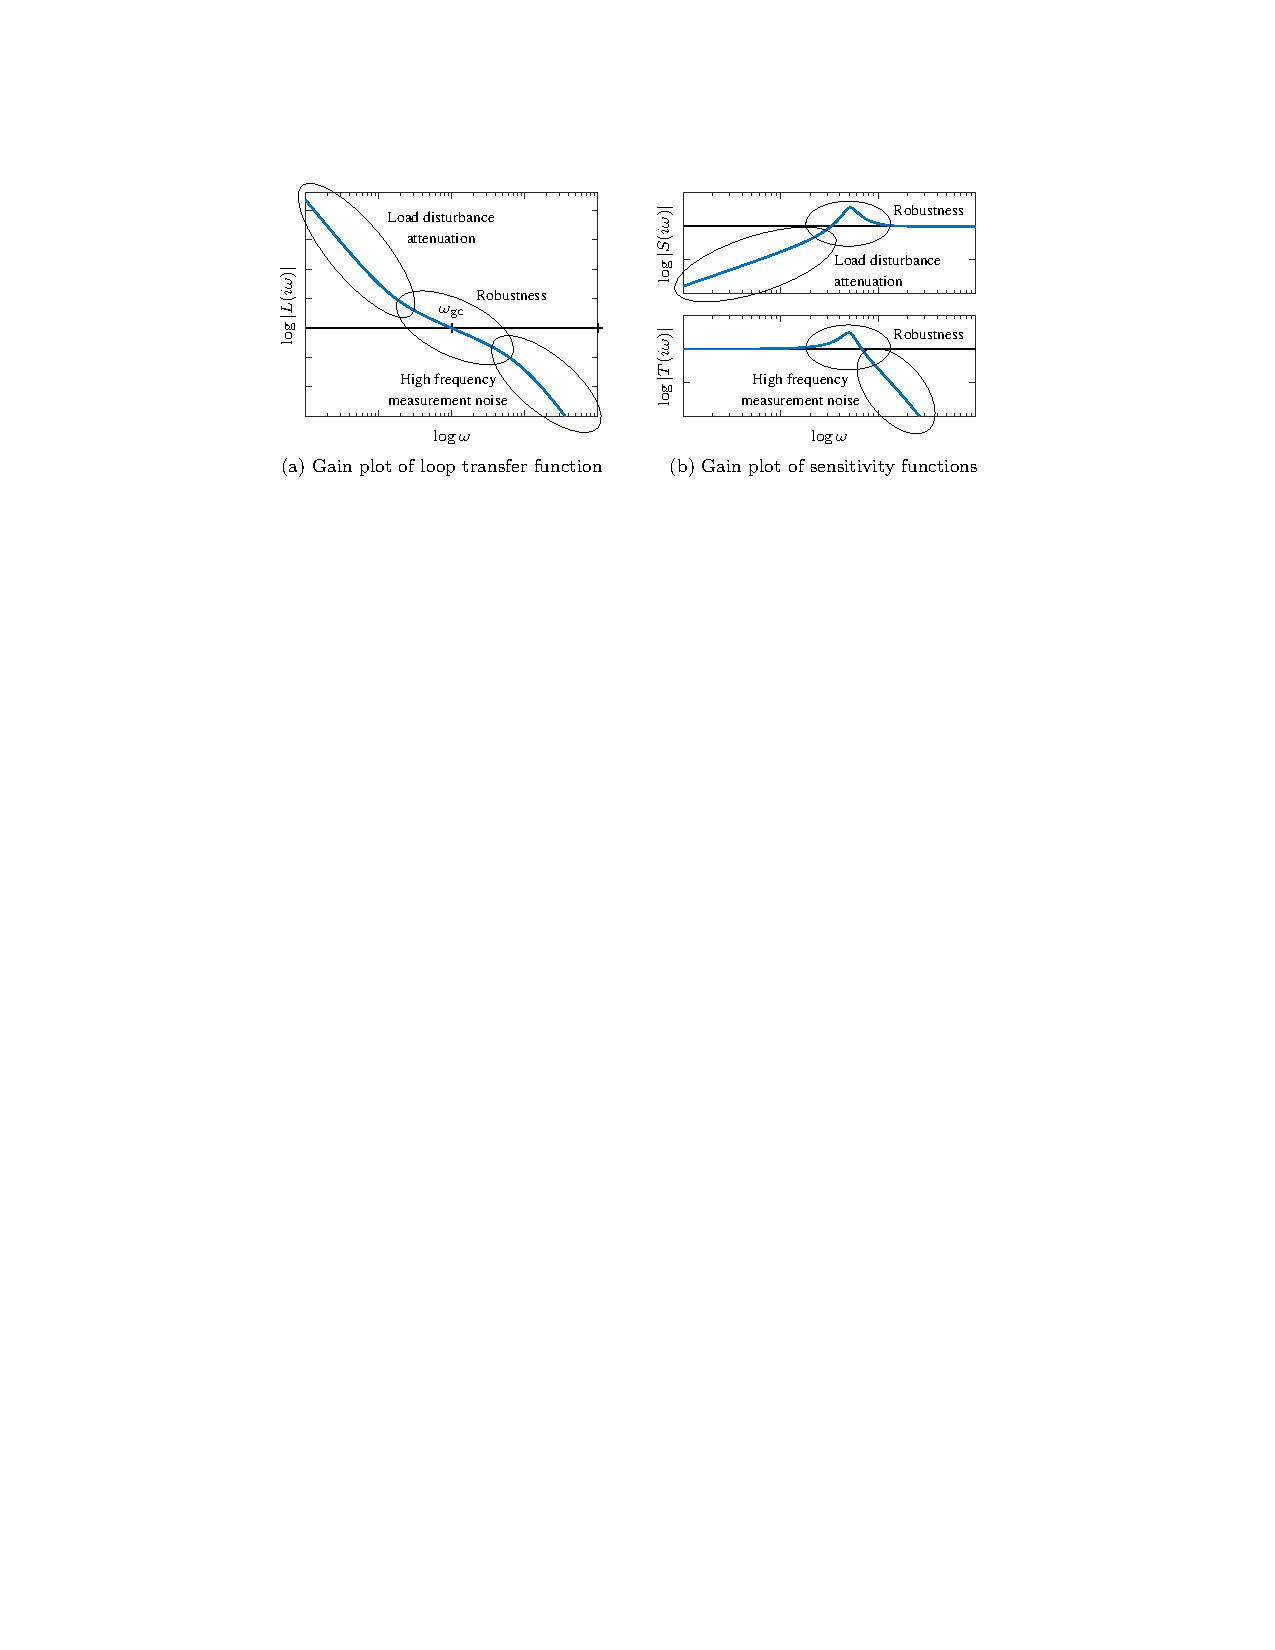
\includegraphics[width=10cm]{figure12.8}\\
	\textbf{Figure 12.8:} Gain plots of the loop transfer function and sensitivity functions.
\end{figure}
\end{frame}


\begin{frame}{Robustness}
\begin{itemize}
	\item The robustness of the system is determined by the shape of the loop transfer function around the crossover frequency $\omega_{gc}$
	\item It is desirable to transition from high loop gain at low frequencies to low loop gain quickly, but robustness requirements (expressed by Bode's relations) impose restrictions on how fast the gain can decrease
	\item For a gain curve of constant slope around $\omega_{gc}$, the slope $n_{gc}$ is related to the phase margin $\varphi_m$ (in degrees) by
	\[n_{gc} \approx -2 + \frac{\varphi_m}{90}\]
	for minimum-phase systems
	\item So, a steeper slope gives a smaller phase margin
\end{itemize}
\end{frame}


\SUBCONCEPT{Lead and lag compensation}

\begin{frame}{A simple way to shape loops}
\begin{itemize}
\item One method for loop shaping is to start with the transfer function of the process and add simple compensaters with the transfer function
\[C(s)=k\frac{s+a}{s+b}, \quad a>0, b>0\]
\item This compensator is known as a \textit{lead compensator} if $a<b$ and a \textit{lag compensator} if $a>b$
\item As this transfer function is first-order, it can provide up to $90^\circ$ of phase lead and larger phase lead can be obtained by using a higher-order lead compensator
\[C(s)=k\frac{(s+a)^n}{(s+b)^n}, \quad a<b\]
\end{itemize}
\end{frame}

\begin{frame}{Relation to PI and PD controllers}
\begin{itemize}
	\item A PD controller with filtering is the same as a lead compensator
	\item The filter for the derivative action in a PID controller to limit high-frequency gain has the same effect as the pole at $s=b$ in the lead compensator
	\item A PI controller is a special case of a lag compensator with $b=0$
\end{itemize}
\end{frame}


\begin{frame}{Effect of lead and lag compensation}
\begin{itemize}
	\item Lead compensation increases the gain at high frequencies and improves the phase margin
	\item Lag compensation increases the gain at low frequencies and can be used to improve tracking performance and low-frequency disturbance attenuation
\end{itemize}

\begin{figure}
	\centering
	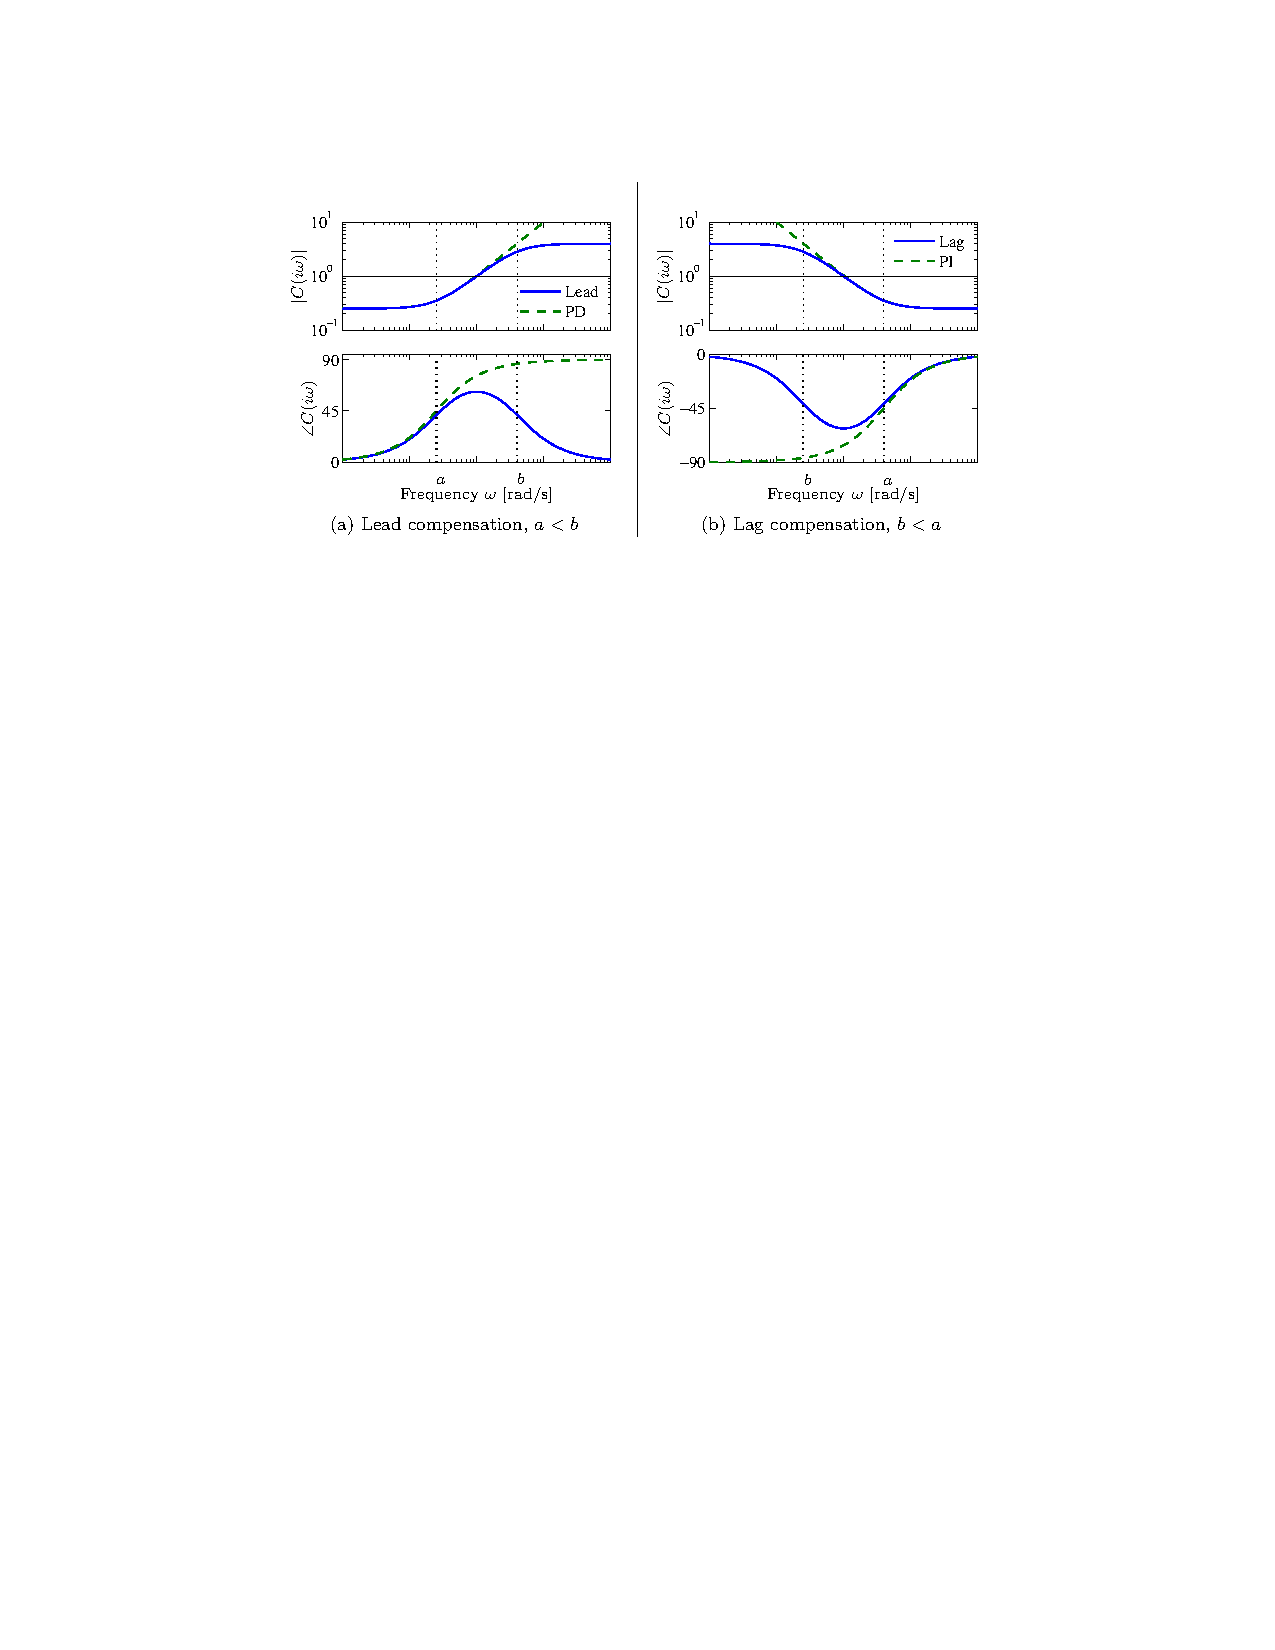
\includegraphics[width=9cm]{figure12.9}\\
	\vspace{-0.2cm}
	\textbf{Figure 12.9:} Frequency response for lead and lag compensators.
\end{figure}
\end{frame}


\SUMMARYFRAME
\FINALE

\end{document}
